\documentclass[11pt]{exam}

\usepackage{amsmath}
\usepackage{graphicx}
\usepackage{geometry}
\usepackage{etoolbox}
\BeforeBeginEnvironment{choices}{\par\nopagebreak\minipage{\linewidth}}
\AfterEndEnvironment{choices}{\endminipage}
\geometry{
a4paper,
total={185mm,257mm},
left=10mm,
top=25mm,
bottom=10mm
}

\begin{document}
\setlength{\voffset}{-0.5in}
\setlength{\headsep}{5pt}

\fbox{\fbox{\parbox{8cm}{\centering
\vspace{2mm}
Testat - Versuch K - Radioaktivitaet - 1
\vspace{2mm}
}}}
\hspace{2mm}
\makebox[0.25\textwidth]{Name:\enspace\hrulefill} \hspace{5mm}
\makebox[0.2\textwidth]{Datum:\enspace\hrulefill}
\vspace{4mm}

\begin{questions}

\question 3000 Imp/min (Impulse pro Minute) entsprechen:	* 10800 Imp/s	* 3 Imp/s	* 300 Imp/s	* 10800 Imp/h	* 3 Imp/h	* 180000 Imp/h

\begin{choices}
	\choice nur 1 und 5 sind richtig
	\choice nur 3 ist richtig
	\choice nur 6 ist richtig (correct)
	\choice nur 3 und 6 sind richtig
	\choice nur 2 und 4 sind richtig
\end{choices}

\vspace{3mm}\question Im unten dargestellten Diagramm ist die Aktivität eines radioaktiven Präparates in Abhängigkeit von der Zeit dargestellt. Wie groß ist die Halbwertszeit? 

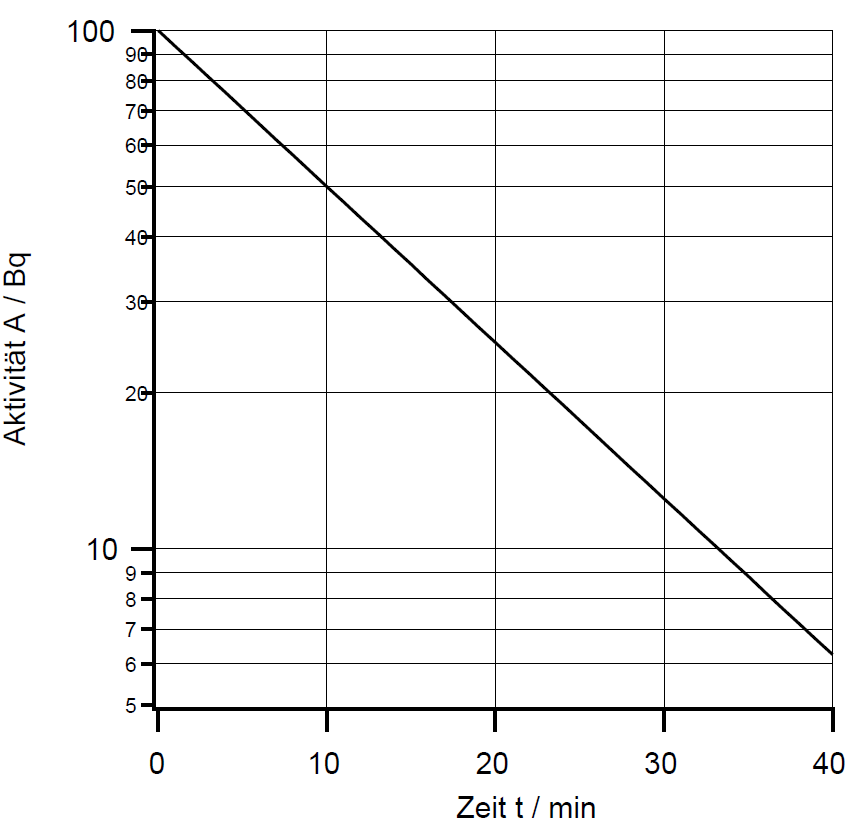
\includegraphics[width=0.5\textwidth]{../../../questions/K/images/zerfallsgesetz.png}

\begin{choices}
	\choice etwa 5 min
	\choice etwa 100 min
	\choice etwa 10 min (correct)
	\choice etwa 20 min
	\choice etwa 1 min
\end{choices}

\vspace{3mm}\question Die Halbwertszeit von Jod-131 beträgt ca. 8 Tage. Die Anfangsaktivität beträgt 500 Bq. Wie groß ist die Aktivität nach 10 Tagen?

\begin{choices}
	\choice 1290 Bq
	\choice 250 Bq
	\choice 210 Bq (correct)
	\choice 500 Bq
	\choice 125 Bq
\end{choices}

\vspace{3mm}\question Welche Aussage ist falsch?

\begin{choices}
	\choice Elektronen verlieren ihre Energie nur durch Stoßionisationen. (correct)
	\choice Stoßionisation kommt z.B. in einem Geiger-Müller-Zählrohr vor.
	\choice Gammastrahlung kann z.B. durch den Photoeffekt absorbiert werden.
	\choice Beim Comptoneffekt entsteht Sekundärstrahlung.
	\choice  Beim Photoeffekt entsteht Sekundärstrahlung.
\end{choices}

\vspace{3mm}\question Das Schwächungsgesetz beschreibt den Zusammenhang zwischen Intensität der Strahlung und Absorberdicke. Der Zusammenhang zwischen diesen Größen ist ...

\begin{choices}
	\choice keine der Antworten ist richtig.
	\choice exponentiell. (correct)
	\choice proportional.
	\choice antiproportional.
	\choice quadratisch.
\end{choices}

\vspace{3mm}\end{questions}

\end{document}
